%Writeup for ENGR202 Lab {INSERT LAB #}
%If editing in vim/vi please insert your own line breaks! This will help keep the file cleaner and easier to edit.

%::Collaboration etiquette::
%In order to better identify changes
%please surround all edits with your
%name as follows:

%BEGIN Zach
%END Zach

%LaTeX will ignore line breaks so to denote
%changes in the middle of a line begin the
%edits on a new line after your name tag
%and then continue with the original on
%the next line following your ending name
%tag.



\documentclass{article}
\usepackage{graphicx}
\graphicspath{ {images/} }

%Change # to correct lab number!
\title{Chapter 5 Lab Writeup}
\author{Zach Thompson, Simon Hannes, Kyle Peterson}
\begin{document}

\maketitle{}

\section*{Overview}
\paragraph{}
%BEGIN ZACH
The purpose of this lab was to examine different types of filters and how they react to changing frequencies.
Three different filters were given to classify.

%END ZACH


\section*{Process}
%BEGIN KYLE
\paragraph{}
To determine the filter type of each circuit we are taking two measurements on the osciloscope at each of the 
10 frequencies in the table. The voltage is measured across the capacitor, inductor, and resistor for the 
respective mystery filters one, two, and three. The time shift is also recorded to be able to use with 
calculating the phase shift. The corner frequencies can be found using the data collected and the equation 
$ V_{out} = (7.07)   V_{in}$ . For the third filter two corner frequencies are found. The data is graphed on 
a logarithmic scaled graph.
%END KYLE

\section*{Results}
\paragraph{}
The corner frequency is found when the output voltage is equal to 5.656V.
\newline
Low Pass Filter: $F_{3db} = 1.7kHz, Phase Shift = 48.96^{\circ}$
\newline
High Pass Filter: $F_{3db} = 23kHz, Phase Shift = 66.24^{\circ}$
\newline
Band Pass Filter: $F_{3db} = 1.1kHz, Phase Shift = 39.6^{\circ}$
and $F_{3db} = 1.5kHz, Phase Shift = 54^{\circ}$

%ZACH ADDING GRAPHS
\begin{figure}[!ht]
\caption{Band Pass Filter}
\begin{center}
\begin{tabular}{|c|c|c|c|c|c|}
\hline
VIN (V)&Freq (Hz)&VOUT(V)&Period (sec)&Time Shift&Phase Shift (degree)\\
\hline
8&10&0&0.1&25000&90\\
\hline
8&30&0.14&0.033333333&9000&97.2\\
\hline
8&100&.49&0.01&2480&89.28\\
\hline
8&300&1.4&0.003333333&760&82.08\\
\hline
8&1000&5.28&0.001&116&41.76\\
\hline
8&3000&4.56&0.000333333&46&49.68\\
\hline
8&10000&1.28&0.0001&23&82.8\\
\hline
8&30000&0.4&3.33333E-05&8.6&92.88\\
\hline
8&100000&0.074&0.00001&2.4&86.4\\
\hline
8&300000&0.5&3.33333E-06&0.92&99.36\\
\hline
\end{tabular}

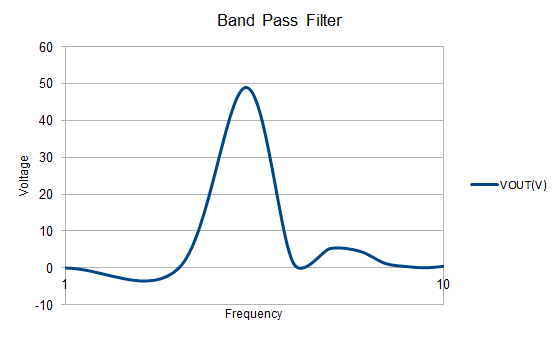
\includegraphics{BandPass.png}
\end{center}
\end{figure}


\begin{figure}[!ht]
\caption{High Pass Filter}
\begin{center}
\begin{tabular}{|c|c|c|c|c|c|}
\hline
VIN (V)&Freq (Hz)&VOUT(V)&Period (sec)&Time Shift&Phase Shift (degree)\\
\hline
8&10&0&0.1&25000&90\\
\hline
8&30&0.14&0.033333333&9000&97.2\\
\hline
8&100&.49&0.01&2480&89.28\\
\hline
8&300&1.4&0.003333333&760&82.08\\
\hline
8&1000&5.28&0.001&116&41.76\\
\hline
8&3000&4.56&0.000333333&46&49.68\\
\hline
8&10000&1.28&0.0001&23&82.8\\
\hline
8&30000&0.4&3.33333E-05&8.6&92.88\\
\hline
8&100000&0.074&0.00001&2.4&86.4\\
\hline
8&300000&0.5&3.33333E-06&0.92&99.36\\
\hline
\end{tabular}

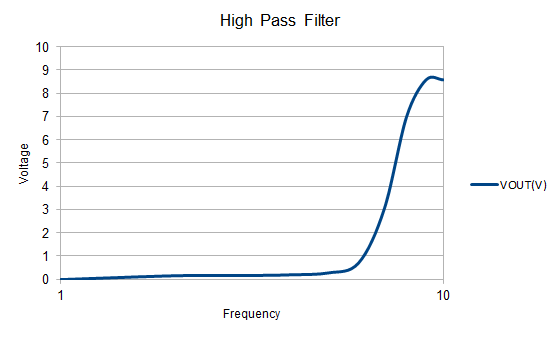
\includegraphics{HighPass.png}
\end{center}
\end{figure}


\begin{figure}[!ht]
\caption{Low Pass Filter}
\begin{center}
\begin{tabular}{|c|c|c|c|c|c|}
\hline
VIN (V)&Freq (Hz)&VOUT(V)&Period (sec)&Time Shift (micro s)&Phase Shift (degree)\\
\hline
8&10&8&0.1&0&0\\
\hline
8&30&8&0.033333333&0&0\\
\hline
8&100&7.8&0.01&0&0\\
\hline
8&300&7&0.003333333&120&12.96\\
\hline
8&1000&6.6&0.001&88&31.68\\
\hline
8&3000&3.6&0.000333333&64&69.12\\
\hline
8&10000&1.2&0.0001&24&86.4\\
\hline
8&30000&0.48&3.33333E-05&8&86.4\\
\hline
8&100000&0.15&0.00001&2.2&79.2\\
\hline
8&300000&0.074&3.33333E-06&0.48&51.84\\
\hline
\end{tabular}

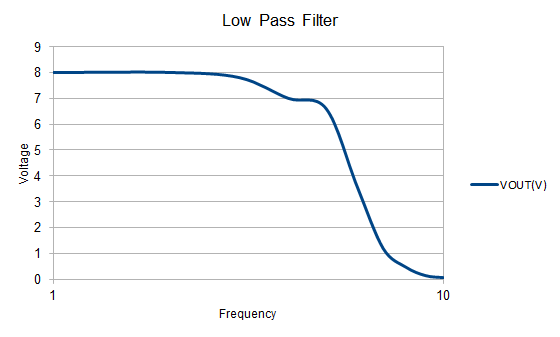
\includegraphics{LowPass.png}
\end{center}
\end{figure}

\clearpage
%END ZACH ADD GRAPHS

\section*{Conclusion}
%BEGIN KYLE
\paragraph{}
The first filter is a low pass filter. We can determine this from just the first value of $10Hz$ which has a 
$V_{out} = V_{in}$ with a phase shift of zero. Then as the frequency increases $V_{out}$ decreases. That
voltage to frequency response is what would be expected from a low pass filter.
\paragraph{}
The second filter is a high pass filter. Unlike the first filter it starts with a $V_{out} = 0$ at a low frequency
 then increases until $V_{out} = V_{in}$ at a high frequency. We can conclude that the result is as would be 
 expeced from a high pass filter.
 \paragraph{}
 The third and final filter is a band pass filter. A Band pass has low voltage outputs at bioth low and high frequencies 
 with a notable peak around the center. Our data actually has two peaks, one being much smaller than the other. This 
 is most likely caused by some sort of wrap around in relation to the phase response of the circuit. We can then conclude
 that the filter is a band pass because the voltages at the low and high frequencies was zero.
 %END KYLE

\section*{Study Questions}

\end{document}
